\section{The proof interface}
\label{sec:barrel-interface}

A long import gives no sign of life, because Lean publishes a command's messages only when
the command has finished; and the source text does not say how many obligations remain,
which operation they belong to, or whether a script that looks complete still admits some of
its goals.
Loading \barrel{} therefore registers a panel in Lean's infoview that reports on both.
It is strictly observational: no theorem's construction or checking depends on it, and it
can be switched off, so it sits outside the trust argument of
\Cref{subsec:barrel-automation}.
The three states below are those of the refinement chain of \Cref{sec:barrel-example}, whose
figures they make concrete.

\definecolor{barrelUiBackground}{RGB}{253,248,237}
\definecolor{barrelUiBorder}{RGB}{209,215,208}
\definecolor{barrelUiAuto}{RGB}{105,198,143}
\definecolor{barrelUiHand}{RGB}{7,183,208}
\definecolor{barrelUiSorry}{RGB}{219,153,69}
\definecolor{barrelUiPending}{RGB}{200,209,203}
\definecolor{barrelUiPale}{RGB}{184,217,219}
\definecolor{barrelUiText}{RGB}{0,82,96}
\definecolor{barrelUiLabel}{RGB}{70,123,132}
\definecolor{barrelUiMuted}{RGB}{124,158,163}
\definecolor{barrelUiLegendAuto}{RGB}{164,214,177}
\definecolor{barrelUiLegendHand}{RGB}{104,202,217}
\definecolor{barrelUiLegendSorry}{RGB}{236,178,105}
\definecolor{barrelUiLegendPending}{RGB}{213,219,213}
\definecolor{barrelUiError}{RGB}{196,71,31}
\definecolor{barrelUiBarrel}{RGB}{224,157,35}
\definecolor{barrelUiBarrelDark}{RGB}{87,53,9}

\paragraph*{Loading.}
Each artifact gets a card as soon as it is registered, and its bar fills as the discharger
works through the file, so an import can be watched rather than waited out, as depicted in \Cref{fig:barrel-state-loading}.

\begin{figure}[t]
  \centering
  \tikzsetnextfilename{barrel-state-loading}
  \resizebox{\textwidth}{!}{%
    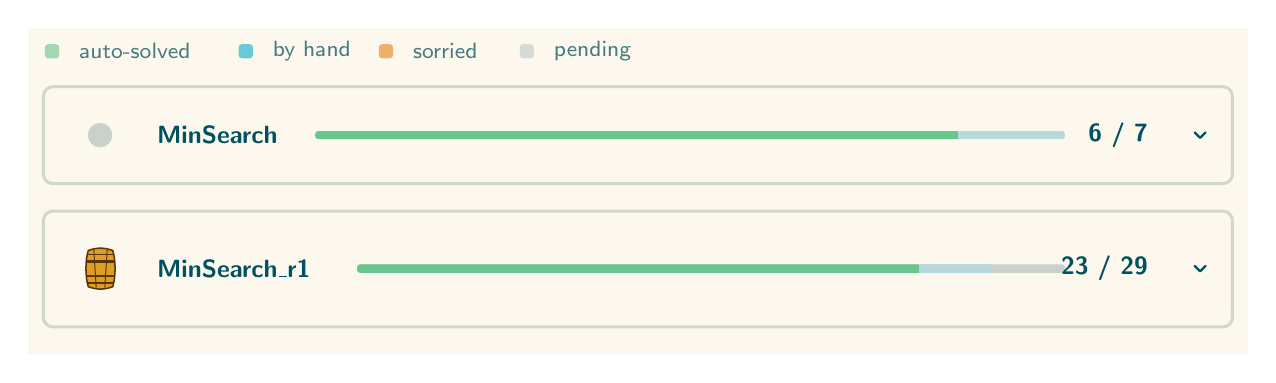
\begin{tikzpicture}[x=1cm,y=1cm,
      legend/.style={font=\fontsize{8.4}{9.4}\selectfont\sffamily,
        text=barrelUiLabel, anchor=west},
      machine/.style={font=\fontsize{9.0}{10}\selectfont\sffamily\bfseries,
        text=barrelUiText, anchor=west},
      meta/.style={font=\fontsize{9.0}{10}\selectfont\sffamily\bfseries,
        text=barrelUiText, anchor=east},
      card/.style={draw=barrelUiBorder, fill=barrelUiBackground,
        rounded corners=.12cm, line width=1.1pt}]
      \useasboundingbox (0,0) rectangle (15.5,4.15);
      \fill[barrelUiBackground] (0,0) rectangle (15.5,4.15);

      \path[fill=barrelUiLegendAuto, rounded corners=.04cm]
        (.22,3.76) rectangle ++(.18,.18);
      \node[legend] at (.53,3.85) {auto-solved};
      \path[fill=barrelUiLegendHand, rounded corners=.04cm]
        (2.68,3.76) rectangle ++(.18,.18);
      \node[legend] at (2.99,3.85) {by hand};
      \path[fill=barrelUiLegendSorry, rounded corners=.04cm]
        (4.46,3.76) rectangle ++(.18,.18);
      \node[legend] at (4.77,3.85) {sorried};
      \path[fill=barrelUiLegendPending, rounded corners=.04cm]
        (6.25,3.76) rectangle ++(.18,.18);
      \node[legend] at (6.56,3.85) {pending};

      \path[card] (.20,2.17) rectangle (15.30,3.40);
      \fill[barrelUiPending] (.92,2.785) circle (.155);
      \node[machine] at (1.52,2.785) {MinSearch};
      \begin{scope}
        \clip[rounded corners=.045cm] (3.65,2.73) rectangle (13.18,2.84);
        \fill[barrelUiAuto] (3.65,2.73) rectangle (11.82,2.84);
        \fill[barrelUiPale] (11.82,2.73) rectangle (13.18,2.84);
      \end{scope}
      \node[meta] at (14.35,2.785) {6 / 7};
      \draw[barrelUiText, line width=.8pt, line cap=round, line join=round]
        (14.82,2.82) -- (14.89,2.75) -- (14.96,2.82);

      \path[card] (.20,.35) rectangle (15.30,1.82);
      \path[fill=barrelUiBarrel, draw=barrelUiBarrelDark, line width=.55pt]
        (.77,.86) .. controls (.73,.98) and (.73,1.20) .. (.77,1.32)
        .. controls (.88,1.36) and (.97,1.36) .. (1.08,1.32)
        .. controls (1.12,1.20) and (1.12,.98) .. (1.08,.86)
        .. controls (.97,.82) and (.88,.82) .. cycle;
      \draw[barrelUiBarrelDark, line width=.55pt] (.77,1.27) -- (1.08,1.27);
      \draw[barrelUiBarrelDark, line width=.8pt] (.75,1.18) -- (1.10,1.18);
      \draw[barrelUiBarrelDark, line width=.8pt] (.75,1.00) -- (1.10,1.00);
      \draw[barrelUiBarrelDark, line width=.55pt] (.77,.91) -- (1.08,.91);
      \draw[barrelUiBarrelDark, line width=.35pt] (.87,.85) -- (.84,1.33);
      \draw[barrelUiBarrelDark, line width=.35pt] (.98,.85) -- (1.01,1.33);

      \node[machine] at (1.52,1.09) {MinSearch\_r1};
      \begin{scope}
        \clip[rounded corners=.045cm] (4.18,1.035) rectangle (13.18,1.145);
        \fill[barrelUiPending] (4.18,1.035) rectangle (13.18,1.145);
        \fill[barrelUiAuto] (4.18,1.035) rectangle (11.32,1.145);
        \fill[barrelUiPale] (11.32,1.035) rectangle (12.25,1.145);
      \end{scope}
      \node[meta] at (14.35,1.09) {23 / 29};
      \draw[barrelUiText, line width=.8pt, line cap=round, line join=round]
        (14.82,1.125) -- (14.89,1.055) -- (14.96,1.125);
    \end{tikzpicture}%
  }
  \caption{Both bars are updated in
    real time: green is the goals the automation has already discharged, pale blue those
    parsed but not yet decided, and the gray remainder those still to be parsed. A gray
    status disc marks an artifact left pending while the rest of the file is checked.}
  \label{fig:barrel-state-loading}
\end{figure}

\paragraph*{Missing blocks, and admitted ones.}
Once the import is over the card shows one cell per goal, grouped by source operation, and
separates two situations that a source file alone does not.
A script may leave obligations without a \leaninl{next} block, in which case their cells stay
gray (\Cref{fig:barrel-state-missing}\,(a)); or it may provide every block and close some of
them with \leaninl{sorry}, in which case those cells are marked and left out of the proved
count (\Cref{fig:barrel-state-missing}\,(b)).
Without the distinction, a syntactically complete development would look finished; the
guarantee itself rests on the axiom check of \Cref{sec:barrel-atelier-comparison}.
When blocks are missing, an action inserts a \leaninl{sorry}-closed skeleton for them, in the
order \leaninl{prove_obligations_of} consumes the goals, which is not the order the map
displays them.

\begin{figure}[t]
  \centering
  \tikzsetnextfilename{barrel-state-missing}
  \resizebox{\textwidth}{!}{%
    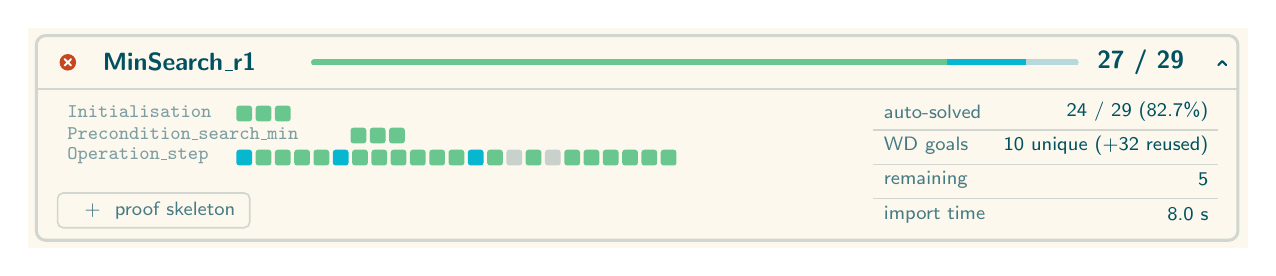
\begin{tikzpicture}[x=1cm,y=1cm,
      machine/.style={font=\fontsize{8.8}{9.8}\selectfont\sffamily\bfseries,
        text=barrelUiText, anchor=west},
      meta/.style={font=\fontsize{8.8}{9.8}\selectfont\sffamily\bfseries,
        text=barrelUiText, anchor=east},
      operation/.style={font=\fontsize{7.2}{8.2}\selectfont\ttfamily,
        text=barrelUiMuted, anchor=west},
      stat/.style={font=\fontsize{7.3}{8.4}\selectfont\sffamily,
        text=barrelUiLabel, anchor=west},
      value/.style={font=\fontsize{7.3}{8.4}\selectfont\sffamily,
        text=barrelUiText, anchor=east},
      card/.style={draw=barrelUiBorder, fill=barrelUiBackground,
        rounded corners=.12cm, line width=1.1pt},
      divider/.style={draw=barrelUiBorder, line width=.45pt}]
      \useasboundingbox (0,0) rectangle (15.5,2.80);
      \fill[barrelUiBackground] (0,0) rectangle (15.5,2.80);
      \path[card] (.11,.10) rectangle (15.37,2.70);
      \draw[divider] (.11,2.02) -- (15.37,2.02);

      \fill[barrelUiError] (.51,2.36) circle (.105);
      \draw[white, line width=.7pt, line cap=round]
        (.47,2.32) -- (.55,2.40) (.47,2.40) -- (.55,2.32);
      \node[machine] at (.83,2.36) {MinSearch\_r1};
      \begin{scope}
        \clip[rounded corners=.035cm] (3.60,2.32) rectangle (13.35,2.40);
        \fill[barrelUiAuto] (3.60,2.32) rectangle (11.67,2.40);
        \fill[barrelUiHand] (11.67,2.32) rectangle (12.68,2.40);
        \fill[barrelUiPale] (12.68,2.32) rectangle (13.35,2.40);
      \end{scope}
      \node[meta] at (14.81,2.36) {27 / 29};
      \draw[barrelUiText, line width=.75pt, line cap=round, line join=round]
        (15.12,2.325) -- (15.17,2.375) -- (15.22,2.325);

      \node[operation] at (.38,1.73) {Initialisation};
      \foreach[count=\i from 0] \c in {
          barrelUiAuto,barrelUiAuto,barrelUiAuto}{
        \path[fill=\c, rounded corners=.035cm]
          ({2.65+.245*\i},1.61) rectangle ++(.20,.20);}
      \node[operation] at (.38,1.45) {Precondition\_search\_min};
      \foreach[count=\i from 0] \c in {
          barrelUiAuto,barrelUiAuto,barrelUiAuto}{
        \path[fill=\c, rounded corners=.035cm]
          ({4.10+.245*\i},1.33) rectangle ++(.20,.20);}
      \node[operation] at (.38,1.17) {Operation\_step};
      \foreach[count=\i from 0] \c in {
          barrelUiHand,barrelUiAuto,barrelUiAuto,barrelUiAuto,
          barrelUiAuto,barrelUiHand,barrelUiAuto,barrelUiAuto,
          barrelUiAuto,barrelUiAuto,barrelUiAuto,barrelUiAuto,
          barrelUiHand,barrelUiAuto,barrelUiPending,barrelUiAuto,
          barrelUiPending,barrelUiAuto,barrelUiAuto,barrelUiAuto,
          barrelUiAuto,barrelUiAuto,barrelUiAuto}{
        \path[fill=\c, rounded corners=.035cm]
          ({2.65+.245*\i},1.05) rectangle ++(.20,.20);}

      \node[stat] at (10.75,1.73) {auto-solved};
      \node[value] at (15.12,1.73) {24 / 29 (82.7\%)};
      \draw[divider] (10.73,1.50) -- (15.12,1.50);
      \node[stat] at (10.75,1.30) {WD goals};
      \node[value] at (15.12,1.30) {10 unique (+32 reused)};
      \draw[divider] (10.73,1.06) -- (15.12,1.06);
      \node[stat] at (10.75,.87) {remaining};
      \node[value] at (15.12,.87) {5};
      \draw[divider] (10.73,.63) -- (15.12,.63);
      \node[stat] at (10.75,.43) {import time};
      \node[value] at (15.12,.43) {8.0 s};

      \path[draw=barrelUiBorder, fill=barrelUiBackground,
        rounded corners=.07cm, line width=.6pt] (.38,.26) rectangle (2.82,.70);
      \node[font=\fontsize{7.3}{8.4}\selectfont\sffamily,
        text=barrelUiLabel, anchor=west] at (.60,.48)
        {+\hspace{.18cm}proof skeleton};
    \end{tikzpicture}%
  }
  \par\smallskip
  {\small (a) two obligations without a \texttt{next} block}
  \par\medskip
  \tikzsetnextfilename{barrel-state-sorry}
  \resizebox{\textwidth}{!}{%
    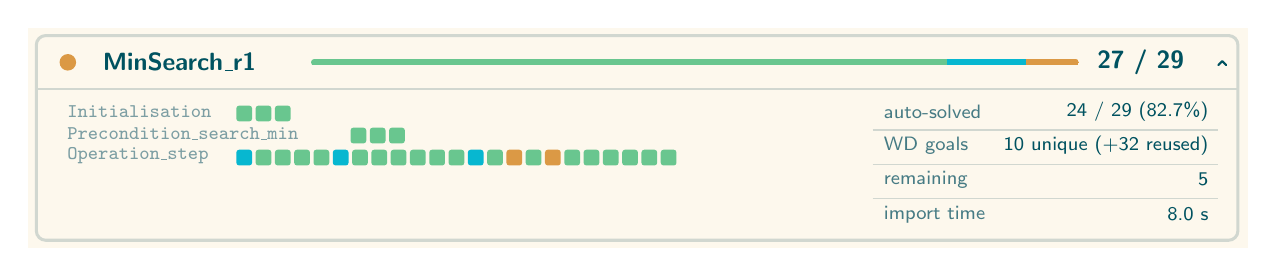
\begin{tikzpicture}[x=1cm,y=1cm,
      machine/.style={font=\fontsize{8.8}{9.8}\selectfont\sffamily\bfseries,
        text=barrelUiText, anchor=west},
      meta/.style={font=\fontsize{8.8}{9.8}\selectfont\sffamily\bfseries,
        text=barrelUiText, anchor=east},
      operation/.style={font=\fontsize{7.2}{8.2}\selectfont\ttfamily,
        text=barrelUiMuted, anchor=west},
      stat/.style={font=\fontsize{7.3}{8.4}\selectfont\sffamily,
        text=barrelUiLabel, anchor=west},
      value/.style={font=\fontsize{7.3}{8.4}\selectfont\sffamily,
        text=barrelUiText, anchor=east},
      card/.style={draw=barrelUiBorder, fill=barrelUiBackground,
        rounded corners=.12cm, line width=1.1pt},
      divider/.style={draw=barrelUiBorder, line width=.45pt}]
      \useasboundingbox (0,0) rectangle (15.5,2.80);
      \fill[barrelUiBackground] (0,0) rectangle (15.5,2.80);
      \path[card] (.11,.10) rectangle (15.37,2.70);
      \draw[divider] (.11,2.02) -- (15.37,2.02);

      \fill[barrelUiSorry] (.51,2.36) circle (.105);
      \node[machine] at (.83,2.36) {MinSearch\_r1};
      \begin{scope}
        \clip[rounded corners=.035cm] (3.60,2.32) rectangle (13.35,2.40);
        \fill[barrelUiAuto] (3.60,2.32) rectangle (11.67,2.40);
        \fill[barrelUiHand] (11.67,2.32) rectangle (12.68,2.40);
        \fill[barrelUiSorry] (12.68,2.32) rectangle (13.35,2.40);
      \end{scope}
      \node[meta] at (14.81,2.36) {27 / 29};
      \draw[barrelUiText, line width=.75pt, line cap=round, line join=round]
        (15.12,2.325) -- (15.17,2.375) -- (15.22,2.325);

      \node[operation] at (.38,1.73) {Initialisation};
      \foreach[count=\i from 0] \c in {
          barrelUiAuto,barrelUiAuto,barrelUiAuto}{
        \path[fill=\c, rounded corners=.035cm]
          ({2.65+.245*\i},1.61) rectangle ++(.20,.20);}
      \node[operation] at (.38,1.45) {Precondition\_search\_min};
      \foreach[count=\i from 0] \c in {
          barrelUiAuto,barrelUiAuto,barrelUiAuto}{
        \path[fill=\c, rounded corners=.035cm]
          ({4.10+.245*\i},1.33) rectangle ++(.20,.20);}
      \node[operation] at (.38,1.17) {Operation\_step};
      \foreach[count=\i from 0] \c in {
          barrelUiHand,barrelUiAuto,barrelUiAuto,barrelUiAuto,
          barrelUiAuto,barrelUiHand,barrelUiAuto,barrelUiAuto,
          barrelUiAuto,barrelUiAuto,barrelUiAuto,barrelUiAuto,
          barrelUiHand,barrelUiAuto,barrelUiSorry,barrelUiAuto,
          barrelUiSorry,barrelUiAuto,barrelUiAuto,barrelUiAuto,
          barrelUiAuto,barrelUiAuto,barrelUiAuto}{
        \path[fill=\c, rounded corners=.035cm]
          ({2.65+.245*\i},1.05) rectangle ++(.20,.20);}

      \node[stat] at (10.75,1.73) {auto-solved};
      \node[value] at (15.12,1.73) {24 / 29 (82.7\%)};
      \draw[divider] (10.73,1.50) -- (15.12,1.50);
      \node[stat] at (10.75,1.30) {WD goals};
      \node[value] at (15.12,1.30) {10 unique (+32 reused)};
      \draw[divider] (10.73,1.06) -- (15.12,1.06);
      \node[stat] at (10.75,.87) {remaining};
      \node[value] at (15.12,.87) {5};
      \draw[divider] (10.73,.63) -- (15.12,.63);
      \node[stat] at (10.75,.43) {import time};
      \node[value] at (15.12,.43) {8.0 s};
    \end{tikzpicture}%
  }
  \par\smallskip
  {\small (b) the same two obligations closed with \texttt{sorry}}
  \caption{Two states that a source file alone does not distinguish. In (a) the goals have
    no proof block and the insertion action is offered; in (b) the blocks exist but admit
    their goals, so the action disappears while the goals are marked in orange and excluded
    from the proved count.}
  \label{fig:barrel-state-missing}
\end{figure}
\FloatBarrier

\paragraph*{Completion.}
When every obligation has a checked proof the card collapses to a single line, so a
multi-artifact development is read at a glance, and expanding it restores the goal map and
the import statistics
(\Cref{fig:barrel-state-complete}).

\begin{figure}[ht!]
  \centering
  \tikzsetnextfilename{barrel-state-complete}
  \resizebox{\textwidth}{!}{%
    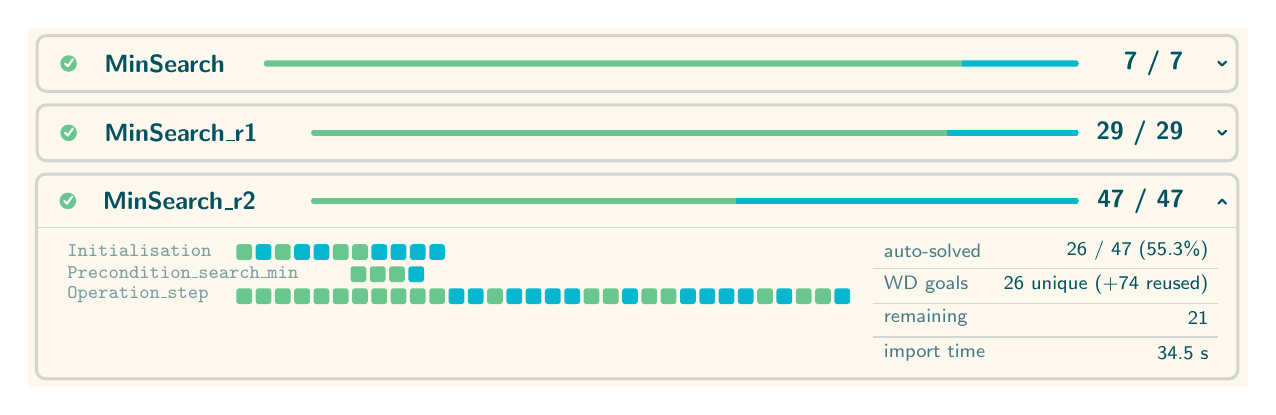
\begin{tikzpicture}[x=1cm,y=1cm,
      machine/.style={font=\fontsize{8.8}{9.8}\selectfont\sffamily\bfseries,
        text=barrelUiText, anchor=west},
      meta/.style={font=\fontsize{8.8}{9.8}\selectfont\sffamily\bfseries,
        text=barrelUiText, anchor=east},
      operation/.style={font=\fontsize{7.2}{8.2}\selectfont\ttfamily,
        text=barrelUiMuted, anchor=west},
      stat/.style={font=\fontsize{7.3}{8.4}\selectfont\sffamily,
        text=barrelUiLabel, anchor=west},
      value/.style={font=\fontsize{7.3}{8.4}\selectfont\sffamily,
        text=barrelUiText, anchor=east},
      card/.style={draw=barrelUiBorder, fill=barrelUiBackground,
        rounded corners=.12cm, line width=1.1pt},
      divider/.style={draw=barrelUiBorder, line width=.45pt}]
      \useasboundingbox (0,0) rectangle (15.5,4.56);

      \fill[barrelUiBackground] (0,0) rectangle (15.5,4.56);

      \foreach \bottom/\top/\cy in {3.75/4.46/4.105,2.87/3.58/3.225}{
        \path[card] (.12,\bottom) rectangle (15.36,\top);
        \fill[barrelUiAuto] (.52,\cy) circle (.105);
        \draw[white, line width=.75pt, line cap=round, line join=round]
          (.475,\cy) -- (.51,{\cy-.035}) -- (.575,{\cy+.055});
        \draw[barrelUiText, line width=.75pt, line cap=round, line join=round]
          (15.12,{\cy+.025}) -- (15.17,{\cy-.025}) --
          (15.22,{\cy+.025});}

      \node[machine] at (.85,4.105) {MinSearch};
      \begin{scope}
        \clip[rounded corners=.035cm] (3.00,4.065) rectangle (13.35,4.145);
        \fill[barrelUiAuto] (3.00,4.065) rectangle (11.87,4.145);
        \fill[barrelUiHand] (11.87,4.065) rectangle (13.35,4.145);
      \end{scope}
      \node[meta] at (14.80,4.105) {7 / 7};

      \node[machine] at (.85,3.225) {MinSearch\_r1};
      \begin{scope}
        \clip[rounded corners=.035cm] (3.60,3.185) rectangle (13.35,3.265);
        \fill[barrelUiAuto] (3.60,3.185) rectangle (11.67,3.265);
        \fill[barrelUiHand] (11.67,3.185) rectangle (13.35,3.265);
      \end{scope}
      \node[meta] at (14.80,3.225) {29 / 29};

      \path[card] (.11,.10) rectangle (15.37,2.70);
      \draw[divider] (.11,2.02) -- (15.37,2.02);

      \fill[barrelUiAuto] (.51,2.36) circle (.105);
      \draw[white, line width=.75pt, line cap=round, line join=round]
        (.465,2.36) -- (.50,2.325) -- (.565,2.415);
      \node[machine] at (.83,2.36) {MinSearch\_r2};
      \begin{scope}
        \clip[rounded corners=.035cm] (3.60,2.32) rectangle (13.35,2.40);
        \fill[barrelUiAuto] (3.60,2.32) rectangle (8.99,2.40);
        \fill[barrelUiHand] (8.99,2.32) rectangle (13.35,2.40);
      \end{scope}
      \node[meta] at (14.81,2.36) {47 / 47};
      \draw[barrelUiText, line width=.75pt, line cap=round, line join=round]
        (15.12,2.325) -- (15.17,2.375) -- (15.22,2.325);

      \node[operation] at (.38,1.73) {Initialisation};
      \foreach[count=\i from 0] \c in {
          barrelUiAuto,barrelUiHand,barrelUiAuto,barrelUiHand,
          barrelUiHand,barrelUiAuto,barrelUiAuto,barrelUiHand,
          barrelUiHand,barrelUiHand,barrelUiHand}{
        \path[fill=\c, rounded corners=.035cm]
          ({2.65+.245*\i},1.61) rectangle ++(.20,.20);}
      \node[operation] at (.38,1.45) {Precondition\_search\_min};
      \foreach[count=\i from 0] \c in {
          barrelUiAuto,barrelUiAuto,barrelUiAuto,barrelUiHand}{
        \path[fill=\c, rounded corners=.035cm]
          ({4.10+.245*\i},1.33) rectangle ++(.20,.20);}
      \node[operation] at (.38,1.17) {Operation\_step};
      \foreach[count=\i from 0] \c in {
          barrelUiAuto,barrelUiAuto,barrelUiAuto,barrelUiAuto,
          barrelUiAuto,barrelUiAuto,barrelUiAuto,barrelUiAuto,
          barrelUiAuto,barrelUiAuto,barrelUiAuto,barrelUiHand,
          barrelUiHand,barrelUiAuto,barrelUiHand,barrelUiHand,
          barrelUiHand,barrelUiHand,barrelUiAuto,barrelUiAuto,
          barrelUiHand,barrelUiAuto,barrelUiAuto,barrelUiHand,
          barrelUiHand,barrelUiHand,barrelUiHand,barrelUiAuto,
          barrelUiHand,barrelUiAuto,barrelUiAuto,barrelUiHand}{
        \path[fill=\c, rounded corners=.035cm]
          ({2.65+.245*\i},1.05) rectangle ++(.20,.20);}

      \node[stat] at (10.75,1.73) {auto-solved};
      \node[value] at (15.12,1.73) {26 / 47 (55.3\%)};
      \draw[divider] (10.73,1.50) -- (15.12,1.50);
      \node[stat] at (10.75,1.30) {WD goals};
      \node[value] at (15.12,1.30) {26 unique (+74 reused)};
      \draw[divider] (10.73,1.06) -- (15.12,1.06);
      \node[stat] at (10.75,.87) {remaining};
      \node[value] at (15.12,.87) {21};
      \draw[divider] (10.73,.63) -- (15.12,.63);
      \node[stat] at (10.75,.43) {import time};
      \node[value] at (15.12,.43) {34.5 s};
    \end{tikzpicture}%
  }
  \caption{Completion of the refinement chain, with all obligations discharged.}
  \label{fig:barrel-state-complete}
\end{figure}
\FloatBarrier
